\section{Description of multiple frame implementations}

There are multiple ways to design a variable pitch quadrotor, one of the first considerations is the frame design. 
\\
One possible design solution is a H-frame. The H design can be summarized as simple as having a frame shaped like an H. The advantages with this design is that we can use one central motor with a constant RPM instead of four motors. This will most likely be the most energy efficient solution, however the disadvantage of the central motor is that you probably won't  get the same agility and performance as having four separate motors with the ability to control both pitch and RPM at once. (figure \ref{H})
\\\\
The most common frame design is the X-frame. This design does not favor any specific flight direction as well as being simple and robust. Additionally this standard quad design works well with most flight controllers and autopilot systems. The X design however will require four separate motors, thus mass will be distributed further out on the arms of the quad in comparison to the central motor. Moving mass away from the center of gravity will result in a higher inertia. It is possible that this effect might be negligible in small quadcopters. (figure \ref{X})
\\\\
A third solution could be a plus-design. The design has a preferred flight direction, in opposition to X-frame. It will probably give a lower torque this is due to the orientation of the propellers and them not being able to contribute to torque simultaneously. (figure \ref{Plus})


\begin{figure}[h]
        \centering
        
    \begin{minipage}[t]{0.32\textwidth}
          \centering
            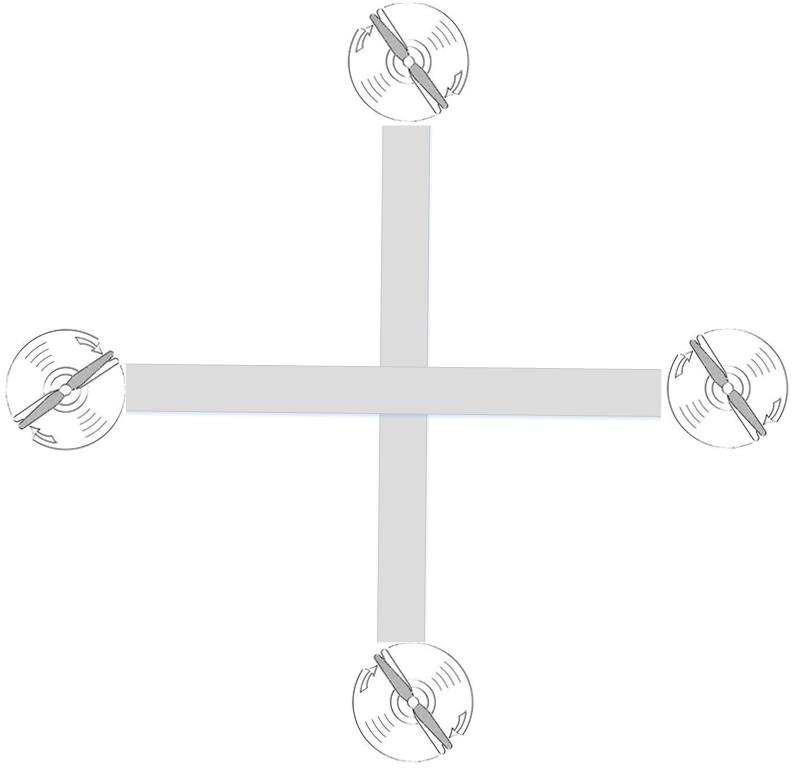
\includegraphics[width = 0.4\textwidth]{VAPIQ-PICTURES/+copter.jpg}
            \caption{Plus-Frame}
            \label{Plus}
    \end{minipage}
            \hfill
    \begin{minipage}[t]{0.32\textwidth}
         \centering
           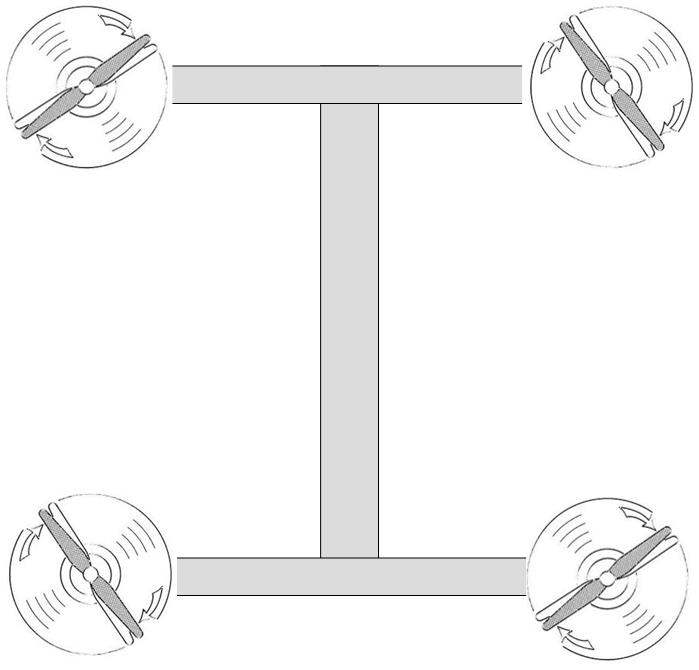
\includegraphics[width = 0.4\textwidth]{VAPIQ-PICTURES/H-copter.jpg}
            \caption{H-Frame}
            \label{H}
    \end{minipage}
            \hfill
    \begin{minipage}[t]{0.32\textwidth}
         \centering
            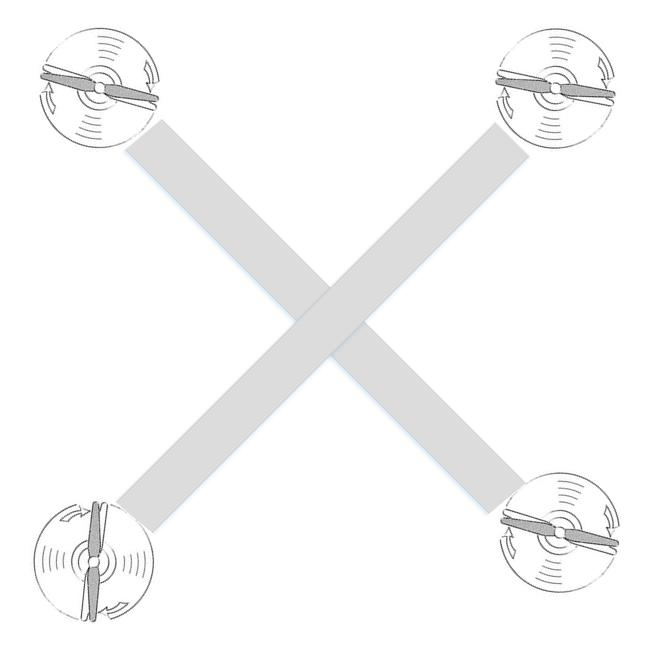
\includegraphics[width = 0.4\textwidth]{VAPIQ-PICTURES/X-copter.jpg}
            \caption{X-Frame}
            \label{X}
    \end{minipage}
\end{figure}






